\documentclass[12pt]{article}

\usepackage[utf8]{inputenc}
\usepackage[T1]{fontenc}
\usepackage[brazil]{babel}
\usepackage{graphicx}
\usepackage{url}
\usepackage{float}
\usepackage{geometry}
\usepackage{caption}
\usepackage{setspace}
\usepackage{booktabs}
\usepackage{multirow}
\usepackage{amsmath}
\usepackage{tikz}
\usetikzlibrary{positioning,arrows.meta,shapes.geometric}
% Figuras: funciona tanto no repo (outputs/figures/) quanto no Overleaf (pasta 'figures/' na raiz)
\graphicspath{{figures/}{outputs/figures/}{./}}
\providecommand{\inst}[1]{\textsuperscript{#1}}
% =========================================================================
% Configurações de Margens e Estilo SBC Inline
% =========================================================================
\geometry{a4paper, top=3.5cm, bottom=2.5cm, left=3.0cm, right=3.0cm}
\usepackage{times}
\setlength{\parindent}{1.27cm}
\setlength{\parskip}{6pt}
\pagestyle{empty}

\makeatletter
\renewcommand{\section}{\@startsection{section}{1}{\z@}%
  {-12pt plus -2pt minus -2pt}{6pt plus 2pt minus 2pt}{\normalfont\large\bfseries}}
\renewcommand{\subsection}{\@startsection{subsection}{2}{\z@}%
  {-12pt plus -2pt minus -2pt}{6pt plus 2pt minus 2pt}{\normalfont\normalsize\bfseries}}
\renewenvironment{abstract}{\centering\begin{minipage}{14.4cm}\small\textbf{Abstract. }\itshape}{\end{minipage}\par\vspace{10pt}}
\newenvironment{resumo}{\centering\begin{minipage}{14.4cm}\small\textbf{Resumo. }\itshape}{\end{minipage}\par\vspace{10pt}}
\makeatother
\DeclareCaptionFont{helvetica}{\fontfamily{phv}\selectfont\small\bfseries}
\captionsetup{font=helvetica,labelsep=period}

% =========================================================================
% Dados do Documento
% =========================================================================
\title{\textbf{Capa Fofa, Conteúdo Sensível: construindo uma base de dados para estudar a discrepância entre a aparência e o conteúdo de romances no Brasil}}

\author{Gabriella de Lima\inst{1}}
\date{}

\begin{document}
\maketitle
\begin{center}
\vspace{-0.8cm}
{\small
$^1$Departamento de Ciência da Computação -- Universidade Federal de Minas Gerais (UFMG)\\
Belo Horizonte -- MG -- Brasil\\[3pt]
\texttt{gabriella.lima@dcc.ufmg.br}
}
\vspace{0.5cm}
\end{center}

% -------------------------------------------------------------------------
\begin{abstract}
A book cover is the first thing a reader sees, and it sets expectations about what is inside. In Brazil, a growing number of romance novels that contain explicit sex, drug and alcohol use, violence or abuse are sold with soft, pastel, cartoon-like covers that look like they were made for teenagers. To study this mismatch between appearance and content, one first needs a dataset that, for each Brazilian edition, pairs the cover and the synopsis with an \emph{independent} description of what the book actually contains. No such dataset existed. This work builds one. We collected 646 Brazilian editions, linked 291 of them to their original works on a reader community platform where people tag books and leave content warnings, and combined five different pieces of evidence into a label that says, for each book, whether there is convergent evidence of sensitive content along four axes: sex, drugs/alcohol, violence and abuse. Two findings stand out. First, in about two thirds of the books that readers flag as sensitive, the Brazilian synopsis says nothing about it. Second, the information readers provide depends heavily on how popular a book is, which means that ``no warning'' cannot be read as ``nothing to warn about''. We explain why this matters, how we dealt with it, and what the resulting dataset can and cannot be used for.
\end{abstract}

\begin{resumo}
A capa é a primeira coisa que o leitor vê, e é ela que cria a expectativa sobre o que há dentro do livro. No Brasil, cresce o número de romances com sexo explícito, uso de drogas e álcool, violência ou abuso que são vendidos com capas suaves, em tons pastéis e estilo de desenho, com aparência de livro para adolescentes. Para estudar essa discrepância entre aparência e conteúdo, é preciso antes ter uma base de dados que, para cada edição brasileira, reúna a capa, a sinopse e uma descrição \emph{independente} do que o livro de fato contém. Essa base não existia. Este trabalho a constrói. Coletamos 646 edições brasileiras, ligamos 291 delas às obras originais em uma plataforma onde leitores marcam livros e registram alertas de conteúdo, e combinamos cinco evidências diferentes em um rótulo que diz, para cada livro, se há indícios convergentes de conteúdo sensível em quatro eixos: sexo, drogas/álcool, violência e abuso. Dois achados se destacam. Primeiro, em cerca de dois terços dos livros que os leitores apontam como sensíveis, a sinopse brasileira não diz nada a respeito. Segundo, a informação que os leitores fornecem depende muito da popularidade do livro, de modo que ``nenhum alerta'' não pode ser lido como ``nada a alertar''. Explicamos por que isso importa, como lidamos com o problema e para que a base resultante pode e não pode ser usada.
\end{resumo}

% =========================================================================
\section{Introdução}
\label{sec:intro}

Quem já entrou em uma livraria sabe que a capa de um livro conta uma história antes mesmo da primeira página. Cores, tipo de letra e estilo de ilustração dizem ao leitor, em um relance, se aquele é um romance leve, um suspense ou um livro infantil \cite{TODO-design-capas}. A capa funciona, portanto, como uma promessa. O problema é que promessas podem não ser cumpridas --- o mesmo fenômeno que a internet batizou de \emph{clickbait}: um título ou uma imagem chamativa que entrega algo bem diferente do que sugeria \cite{TODO-clickbait}.

Nos últimos anos, esse descompasso ganhou uma forma particular no mercado de romances. Impulsionados pela comunidade de leitores do TikTok --- o chamado BookTok ---, livros com cenas de sexo explícito, personagens que abusam de álcool e drogas, violência gráfica ou relações abusivas passaram a ser vendidos com capas ilustradas, coloridas e ``fofas'', em um estilo que historicamente sinalizava literatura juvenil. Chamamos isso de \emph{discrepância entre capa e conteúdo}. E a sinopse, que em tese deveria corrigir a primeira impressão, muitas vezes não o faz: como veremos, ela costuma silenciar justamente sobre o que os leitores consideram digno de aviso.

Por que isso importa? Porque crianças e adolescentes também compram e leem esses livros, e a capa é o principal sinal que eles e seus responsáveis usam para julgar se a obra é adequada \cite{TODO-exposicao-conteudo}. No Brasil, a preocupação ganhou peso legal: a Lei nº~15.211/2025, o Estatuto Digital da Criança e do Adolescente, passou a exigir de serviços digitais mecanismos de proteção, controle parental e verificação de idade \cite{TODO-lei15211}. Como a descoberta e a compra de livros acontecem cada vez mais em redes sociais e lojas virtuais \cite{TODO-social-media-livros}, a pergunta ``esta capa representa honestamente este conteúdo?'' deixa de ser apenas uma escolha estética da editora e passa a ser uma questão de informação ao consumidor em ambiente digital.

\subsection*{O que falta para estudar o problema}
Para investigar se há discrepância, e em que medida, é preciso comparar duas coisas: o que a capa sugere e o que o livro contém. A primeira parte é tratável com técnicas de visão computacional. A segunda é mais difícil do que parece. Não podemos confiar na sinopse, porque ela é parte do problema. Não podemos ler centenas de livros. O que podemos fazer é recorrer aos leitores: em plataformas de catalogação social, milhares de pessoas registram, para cada livro que leram, etiquetas (\emph{tags}) sobre tema e tom e, cada vez mais, \emph{alertas de conteúdo} (\emph{content warnings}) --- avisos do tipo ``contém violência sexual'' ou ``contém alcoolismo''. Esses alertas são uma fonte de informação independente da editora.

Usá-los, porém, impõe dois obstáculos que são o cerne técnico deste trabalho:
\begin{enumerate}
  \item \textbf{As plataformas com essa informação são globais e em inglês}, e catalogam os livros pelo título original. Para saber o que os leitores dizem de \emph{Quarta Asa}, é preciso descobrir que ele é a tradução de \emph{Fourth Wing} --- e títulos traduzidos raramente são traduções literais. Ligar a edição brasileira à obra original é um problema conhecido em computação como \emph{resolução de entidades}.
  \item \textbf{Os alertas são escassos e sua ausência não é neutra.} Um livro muito lido acumula dezenas de alertas; um livro pouco lido pode não ter nenhum, não porque seja inofensivo, mas porque ninguém o marcou. Tratar ``sem alerta'' como ``sem conteúdo sensível'' seria um erro sistemático.
\end{enumerate}

\subsection*{O que este trabalho entrega}
Este texto descreve a primeira etapa de um projeto maior. O objetivo aqui não é ainda medir a discrepância, mas \textbf{construir a base de dados que torna essa medição possível} e entender suas limitações. Para isso:
\begin{itemize}
  \item montamos um processo automatizado e reprodutível que coleta edições brasileiras, as liga às obras originais e baixa suas capas;
  \item definimos uma taxonomia de \textbf{quatro eixos de conteúdo sensível} --- sexo, drogas e álcool, violência, abuso e temas de saúde mental --- com um vocabulário explícito em português e em inglês;
  \item criamos um \textbf{rótulo} para cada obra que combina cinco fontes de evidência e que, crucialmente, \emph{admite não saber} quando não há evidência suficiente;
  \item verificamos a robustez desse rótulo e preparamos um protocolo de validação por pessoas.
\end{itemize}

Ao longo do caminho, dois resultados emergem que vão além da construção da base: a confirmação quantitativa de que a sinopse brasileira omite a maior parte dos alertas que os leitores fazem, e a demonstração de que a informação disponível sobre um livro depende muito da sua popularidade. Ambos têm consequências para como qualquer estudo futuro deve ser desenhado.

O restante do texto está organizado assim: a Seção~\ref{sec:fund} apresenta, em linguagem acessível, os conceitos de que precisamos; a Seção~\ref{sec:metodo} explica como a base foi construída; a Seção~\ref{sec:resultados} apresenta o que encontramos e o que isso significa; a Seção~\ref{sec:discussao} discute os limites do que fizemos; e a Seção~\ref{sec:conclusao} conclui.

% =========================================================================
\section{Conceitos e Trabalhos Relacionados}
\label{sec:fund}

\subsection{Obra e edição não são a mesma coisa}
Quando dizemos ``o livro \emph{Fourth Wing}'', podemos estar falando de coisas diferentes: da história criada pela autora, da tradução para o português, ou do objeto físico publicado por uma editora específica com um determinado ISBN e uma determinada capa. A biblioteconomia formalizou essa distinção no modelo FRBR \cite{TODO-frbr}, que separa a \emph{obra} (a criação intelectual) da \emph{manifestação} (a edição concreta). A distinção é essencial para nós: a \textbf{capa} que queremos estudar pertence à edição brasileira, mas os \textbf{alertas dos leitores} descrevem a obra, independentemente da edição. Nossa base precisa, portanto, guardar as duas camadas e saber ligá-las.

\subsection{Como ligar registros que descrevem a mesma coisa}
Descobrir que dois registros em bases diferentes se referem à mesma entidade --- aqui, que uma edição brasileira corresponde a uma obra em um catálogo em inglês --- é chamado de \emph{record linkage} ou resolução de entidades \cite{TODO-record-linkage}. Quando há um identificador comum (o ISBN), a ligação é trivial. Quando não há, é preciso comparar atributos como título e autor, admitindo variações, traduções e erros de digitação. A dificuldade está em ser permissivo o bastante para encontrar o par certo e rigoroso o bastante para não ligar livros diferentes.

\subsection{O que os leitores dizem: folksonomia e alertas de conteúdo}
Plataformas como Goodreads, Skoob e Hardcover permitem que leitores etiquetem livros livremente. Esse conjunto de etiquetas criado de baixo para cima é chamado de \emph{folksonomia} \cite{TODO-folksonomia}. Entre as etiquetas, os \emph{content warnings} formam um vocabulário relativamente padronizado (\emph{sexual content}, \emph{alcoholism}, \emph{domestic abuse}) e, em algumas plataformas, vêm acompanhados do número de leitores que os confirmaram. Isso os torna um sinal de conteúdo mais confiável que a sinopse, com uma ressalva importante: eles só existem para livros que alguém leu e se deu ao trabalho de marcar.

\subsection{Quando a ausência de dado é, ela mesma, informação}
Em estatística, diz-se que um dado faltante é \emph{não aleatório} (MNAR, do inglês \emph{missing not at random}) quando a chance de ele estar ausente depende de algo relacionado ao próprio valor \cite{TODO-mnar}. É o nosso caso: a chance de um livro não ter alertas depende de quantas pessoas o leram, e a popularidade pode estar relacionada ao tipo de conteúdo. Ignorar isso levaria a conclusões enviesadas --- por exemplo, a de que livros de autoras pouco conhecidas são ``mais leves'', quando na verdade são apenas menos marcados.

\subsection{Rótulos imperfeitos: supervisão fraca}
Quando não é viável que pessoas rotulem manualmente todos os dados, uma alternativa é combinar várias regras automáticas imperfeitas em um rótulo único \cite{TODO-weak-supervision}. A ideia central é que, se fontes \emph{independentes} concordam, a chance de erro cai. Há um caso especial relevante para nós: quando só conseguimos observar evidência \emph{positiva} (alguém marcou que há violência) e nunca evidência negativa confiável (ninguém marca ``não há violência''), o rótulo resultante diz respeito apenas a presença de sinal. Na literatura, isso é chamado de aprendizado \emph{positive-unlabelled} \cite{TODO-pu-learning}, e voltaremos a ele porque define o que o nosso rótulo pode e não pode afirmar.

\subsection{Trabalhos relacionados}
A discrepância entre apresentação e conteúdo foi estudada em vídeos (\emph{thumbnails}) e notícias (\emph{clickbait}) \cite{TODO-clickbait}. Em livros, há trabalhos que classificam o gênero a partir da capa \cite{TODO-cover-genre} e que estimam faixa etária a partir do texto \cite{TODO-age-text}. Não encontramos, porém, trabalhos que tratem do mercado brasileiro, que combinem capa, sinopse e alertas de leitores, ou que enfrentem explicitamente a escassez desses alertas. \emph{(Revisão bibliográfica a completar.)}

% =========================================================================
\section{Como a base foi construída}
\label{sec:metodo}

\subsection{A ideia em uma figura}
A Figura~\ref{fig:pipeline} resume o processo. Partimos de listas de busca (autoras, termos, editoras, títulos), consultamos o Google Books para obter edições brasileiras com sinopse e capa, ligamos cada edição à obra correspondente no Hardcover --- uma plataforma de leitores com API aberta --- para obter as etiquetas e alertas, e combinamos tudo em um rótulo por obra. Em paralelo, baixamos e validamos as capas para uso futuro. Cada etapa pode ser interrompida e retomada sem perder trabalho, o que importa porque as APIs têm limites diários de consulta.

\begin{figure}[H]
\centering
\begin{tikzpicture}[
  node distance=7mm and 9mm,
  box/.style={draw, rounded corners=2pt, align=center, font=\footnotesize, minimum width=28mm, minimum height=9mm},
  src/.style={box, fill=gray!12}, saida/.style={box, fill=gray!28},
  arr/.style={-{Latex[length=2mm]}, thick}]
  \node[src] (seed) {Listas de busca\\autoras, editoras,\\títulos, termos};
  \node[src, right=of seed] (gb) {Google Books\\(edições PT-BR:\\sinopse, capa)};
  \node[box, right=of gb] (ponte) {Ligação\\Edição $\leftrightarrow$ Obra};
  \node[src, above=of ponte] (hc) {Hardcover\\(etiquetas e alertas\\dos leitores)};
  \node[box, below=of ponte] (rot) {Rótulo por\\combinação de\\5 evidências};
  \node[box, left=of rot] (cap) {Capas\\download e validação};
  \node[box, right=of rot] (gold) {Validação\\humana cega};
  \node[saida, below=of rot] (ds) {Base de dados\\rotulada};
  \draw[arr] (seed) -- (gb); \draw[arr] (gb) -- (ponte); \draw[arr] (hc) -- (ponte);
  \draw[arr] (ponte) -- (rot); \draw[arr] (gb) |- (cap); \draw[arr] (rot) -- (ds); \draw[arr] (cap) |- (ds);
  \draw[arr, dashed] (gold) -- (rot); \draw[arr, dashed] (gold.south) |- (ds);
\end{tikzpicture}
\caption{Visão geral do processo de construção da base.}
\label{fig:pipeline}
\end{figure}

\subsection{De onde vêm os dados}
As plataformas de leitores mais usadas no Brasil, Goodreads e Skoob, não oferecem acesso programático aberto \cite{TODO-goodreads-api}. Escolhemos o \textbf{Hardcover}, que disponibiliza uma API com etiquetas de gênero, \emph{moods} (o ``clima'' do livro) e alertas de conteúdo, cada um com a contagem de leitores que o confirmou. Como o catálogo do Hardcover é mantido pelos próprios usuários e está majoritariamente em inglês, usamos o \textbf{Google Books} --- cuja API é aberta e cobre bem o mercado brasileiro --- para obter as edições em português, com sinopse, editora, ano, categorias e capa.

\subsection{Quais livros entram: as listas de busca}
\label{sec:seed}
Não é possível coletar ``todos os romances brasileiros''. Construímos, em vez disso, uma amostra intencional, pensada para conter tanto livros que \emph{provavelmente} têm conteúdo sensível quanto livros que \emph{provavelmente} não têm --- porque, para estudar discrepância, precisamos dos dois polos. As buscas foram feitas por quatro caminhos: (i)~\textbf{autoras}, mais de quinhentas, organizadas por subgênero (\emph{new adult}, \emph{dark romance}, comédia romântica, romance esportivo, romantasia, autoras nacionais) e incluindo grupos de \emph{controle} de autoras de ficção leve, juvenil e fantasia sem romance; (ii)~\textbf{termos} de busca, como nomes de gênero (``romance erótico''), tropos (``inimigos para amantes'') e, separadamente, termos de conteúdo (``conteúdo adulto''); (iii)~\textbf{editoras} brasileiras; e (iv)~\textbf{títulos} citados em listas do BookTok. Guardamos, para cada edição, por qual caminho ela entrou.

Esse último detalhe é mais importante do que parece. Se buscamos livros pela expressão ``conteúdo adulto'' e depois usamos a presença dessa expressão na sinopse como evidência de conteúdo adulto, estamos nos enganando: encontramos o que plantamos. Por isso o caminho ``termos de conteúdo'' é tratado como um estrato à parte, e a Seção~\ref{sec:triang} explica como impedimos que ele contamine o rótulo.

Ao todo, as buscas renderam \textbf{646 edições brasileiras} distintas.

\subsection{Ligando a edição brasileira à obra original}
\label{sec:ponte}
Para cada edição, tentamos encontrar a obra correspondente no Hardcover em uma sequência de tentativas, da mais segura à mais arriscada:
\begin{enumerate}
  \item \textbf{Pelo ISBN.} Se o Hardcover conhece a edição brasileira pelo seu código, a ligação é certa. Isso funciona em menos da metade dos casos: plataformas internacionais raramente cadastram edições brasileiras.
  \item \textbf{Pelo catálogo da autora.} Buscamos todas as obras da autora no Hardcover e comparamos o título brasileiro (depois de remover ruído como ``--- o dark romance que conquistou o TikTok'') com os títulos originais e alternativos. A comparação usa duas medidas: uma puramente textual, que funciona quando a tradução é próxima (\emph{Indigo Ridge} / \emph{Aconteceu em Indigo Ridge}), e uma semântica, baseada em um modelo de linguagem multilíngue, que reconhece que \emph{Quarta Asa} e \emph{Fourth Wing} significam a mesma coisa mesmo sem letras em comum. Para evitar confundir volumes de uma mesma série, exigimos que o melhor candidato esteja claramente à frente do segundo.
  \item \textbf{Por busca textual}, como último recurso.
\end{enumerate}
Em todas as etapas há uma verificação de autoria propositalmente rigorosa, que impede, por exemplo, que um livro de \emph{Christina Lauren} seja ligado a um de \emph{Lauren Asher}. E toda ligação que não veio do ISBN é marcada para revisão humana --- preferimos saber onde o processo pode ter errado a fingir que ele é infalível. Os limiares numéricos usados nas comparações foram fixados antes de ver os resultados e estão documentados no código.

\subsection{Os quatro eixos de conteúdo sensível}
\label{sec:taxonomia}
O projeto começou focado no ``nível de \emph{spice}'' --- a intensidade erótica --- mas ficou claro que a preocupação com adequação de conteúdo é mais ampla. Definimos então quatro eixos, descritos na Tabela~\ref{tab:eixos}. Para cada um, escrevemos um vocabulário explícito em duas línguas: os termos que os leitores usam no Hardcover (em inglês) e os termos que aparecem em sinopses brasileiras (em português). O vocabulário completo está no Apêndice~B, e duas escolhas merecem registro. Primeiro, violência sexual (``estupro'', \emph{rape}) conta em dois eixos ao mesmo tempo, porque é simultaneamente conteúdo sexual e tema de abuso. Segundo, palavras genéricas demais, como \emph{war} ou \emph{death}, ficaram de fora do eixo de violência: elas aparecem em qualquer fantasia épica e diriam pouco sobre adequação.

\begin{table}[H]
\centering\small
\caption{Os quatro eixos de conteúdo sensível e exemplos do vocabulário usado para detectá-los.}
\label{tab:eixos}
\begin{tabular}{lp{5.2cm}p{5.2cm}}
\toprule
\textbf{Eixo} & \textbf{Como os leitores marcam (EN)} & \textbf{Como a sinopse diz (PT)} \\
\midrule
1. Sexo e erotismo & \emph{sexual content, explicit, steamy, open door, dark romance, rape} & conteúdo adulto, cenas quentes, +18, erótico, estupro \\
2. Drogas e álcool & \emph{alcohol, alcoholism, drinking, drug use, addiction, overdose} & alcoolismo, embriaguez, bebidas alcoólicas, uso de drogas, dependência química \\
3. Violência & \emph{violence, gun violence, murder, torture, kidnapping, gore} & violência física, tortura, sequestro, cárcere privado, massacre \\
4. Abuso e gatilhos & \emph{abuse, domestic abuse, toxic relationship, self-harm, suicide, stalking} & abuso psicológico, relacionamento tóxico, suicídio, automutilação \\
\bottomrule
\end{tabular}
\end{table}

\subsection{Como chegamos a um rótulo por obra}
\label{sec:triang}
Nenhuma fonte de informação, sozinha, é confiável. A classificação etária do Google Books quase nunca é preenchida. A sinopse suaviza o conteúdo --- é parte do fenômeno que estudamos. As etiquetas dos leitores são ricas para livros populares e inexistentes para os demais. A solução foi fazer cada fonte ``votar'' separadamente e só confiar no resultado quando há convergência. Cinco fontes votam \emph{alto}, \emph{baixo} ou se abstêm: a escala de intensidade erótica derivada das etiquetas; o vocabulário dos quatro eixos nas etiquetas; o vocabulário dos quatro eixos na sinopse brasileira; a classificação etária do Google Books; e os alertas de conteúdo dos leitores.

Os votos são então combinados por um conjunto de regras simples, aplicadas em ordem, que produzem um de quatro rótulos:
\begin{itemize}
  \item \textbf{alto}: há evidência de conteúdo sensível. Chamamos de \emph{forte} quando duas fontes independentes concordam ou há um alerta explícito dos leitores, e de \emph{fraca} quando só uma fonte se manifestou;
  \item \textbf{baixo}: há evidência explícita de que o livro é leve (etiquetas como \emph{closed door} ou ``romance clean'');
  \item \textbf{provavelmente baixo}: nenhuma fonte se manifestou, mas o livro é catalogado como juvenil \emph{e} tem leitores suficientes para que, se houvesse algo a alertar, alguém provavelmente já teria alertado. Este rótulo é uma inferência, não uma medição, e é tratado como tal;
  \item \textbf{indeterminado}: não há evidência suficiente para dizer nada.
\end{itemize}

Três decisões de desenho merecem explicação porque vão contra o instinto de ``preencher todas as linhas''. A primeira é a \textbf{abstenção}: a ausência de evidência nunca vira ``baixo''. Dada a escassez de etiquetas em livros pouco lidos, qualquer outra escolha rotularia como leves exatamente os livros sobre os quais menos sabemos. A segunda é a \textbf{guarda contra circularidade}: se a única evidência de um livro é a sinopse, e esse livro entrou na amostra porque buscamos ``conteúdo adulto'', essa evidência não vale sozinha --- ela foi plantada pela própria busca. A terceira é que geramos também um \textbf{rótulo que ignora a sinopse}. Ele existe para o futuro: se um modelo for treinado para prever conteúdo a partir da sinopse, usar como alvo um rótulo que já leu a sinopse seria trapaça.

\subsection{Como verificamos se o rótulo é confiável}
\label{sec:validacao}
Um rótulo automático precisa ser testado. Fazemos isso de duas maneiras. A primeira é \textbf{humana}: duas pessoas, sem ver o rótulo automático, classificam 96 obras sorteadas de todos os níveis de popularidade, eixo por eixo, e uma amostra das ligações edição--obra é conferida manualmente. Isso permite medir quanto os anotadores concordam entre si e quão frequentemente o rótulo automático acerta. O protocolo está no Apêndice~C e a anotação está em andamento. A segunda é \textbf{interna}: removemos cada fonte de evidência por vez e observamos quanto o rótulo muda (\emph{ablação}); variamos os parâmetros de decisão e observamos a estabilidade (\emph{sensibilidade}); e medimos quanto as fontes concordam entre si quando mais de uma se manifesta.

% =========================================================================
\section{O que encontramos --- e o que isso significa}
\label{sec:resultados}

\subsection{Do que coletamos ao que conseguimos usar}
\label{sec:res-funil}
Das 646 edições coletadas, conseguimos ligar 291 (45\%) a uma obra no Hardcover (Figura~\ref{fig:funil}). O número parece baixo, mas o padrão da perda é mais revelador que a perda em si: três em cada quatro edições encontradas pelo nome da autora foram ligadas, contra apenas uma em cada quatro das encontradas por termos de conteúdo. Em outras palavras, os livros mais explícitos do catálogo brasileiro --- frequentemente de autoras nacionais ou autopublicados --- são justamente os que menos existem na plataforma internacional. Isso tem uma consequência direta: a base final tende a conter mais autoras estrangeiras traduzidas por editoras grandes, e menos do que há de mais ``de nicho'' no mercado nacional. Qualquer conclusão sobre ``o mercado brasileiro'' deve ser lida com essa ressalva.

Após excluir edições anteriores a 2015 e agrupar reedições da mesma obra, a base final tem \textbf{252 obras} em 262 edições, publicadas por 49 editoras.

\begin{figure}[H]
\centering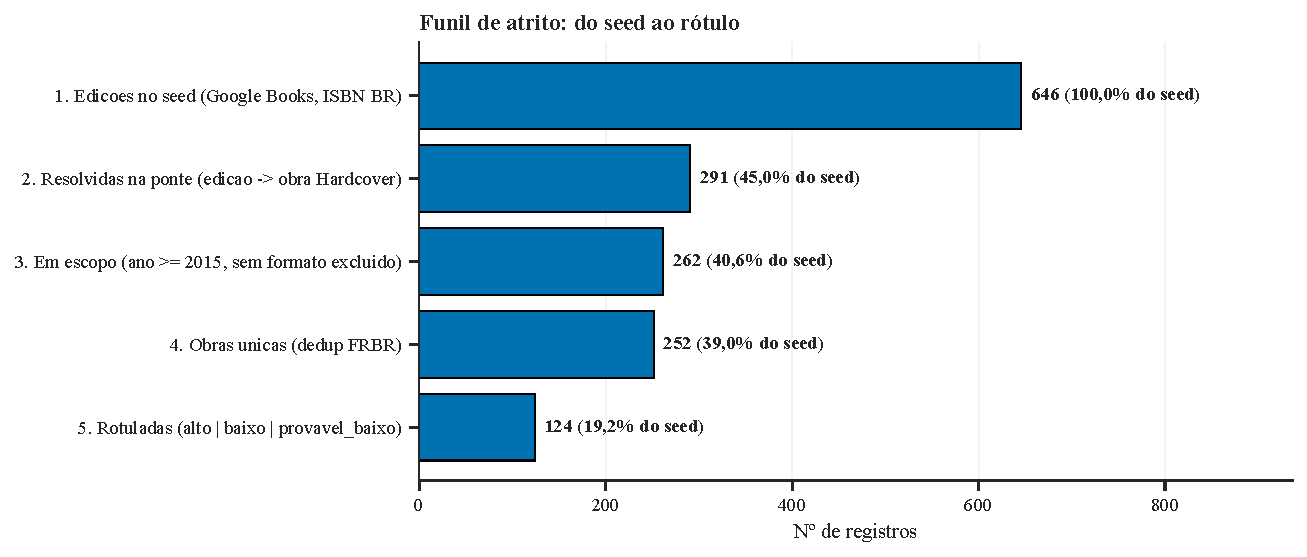
\includegraphics[width=0.95\textwidth]{fig_16_funil.pdf}
\caption{Quantos livros sobrevivem a cada etapa, da coleta ao rótulo definido.}
\label{fig:funil}
\end{figure}

\subsection{A informação dos leitores depende da popularidade}
\label{sec:res-mnar}
Este é, talvez, o resultado que mais condiciona tudo o mais. Dividimos as obras em quatro grupos de igual tamanho, do menos ao mais lido, e contamos quantas têm algum alerta de conteúdo. No grupo menos lido, praticamente nenhuma (1,6\%). No grupo mais lido, mais de dois terços (68\%). A Figura~\ref{fig:cobertura} mostra o mesmo padrão para todos os tipos de etiqueta, e a correlação entre número de leitores e quantidade de etiquetas é altíssima ($\rho = 0{,}91$).

O que isso significa na prática: se um livro pouco lido não tem alerta de violência, não sabemos se é porque não há violência ou porque ninguém o marcou. É exatamente a situação de dado faltante não aleatório descrita na Seção~\ref{sec:fund}, e é a razão pela qual nosso rótulo admite ``indeterminado'' em vez de forçar uma resposta.

\begin{figure}[H]
\centering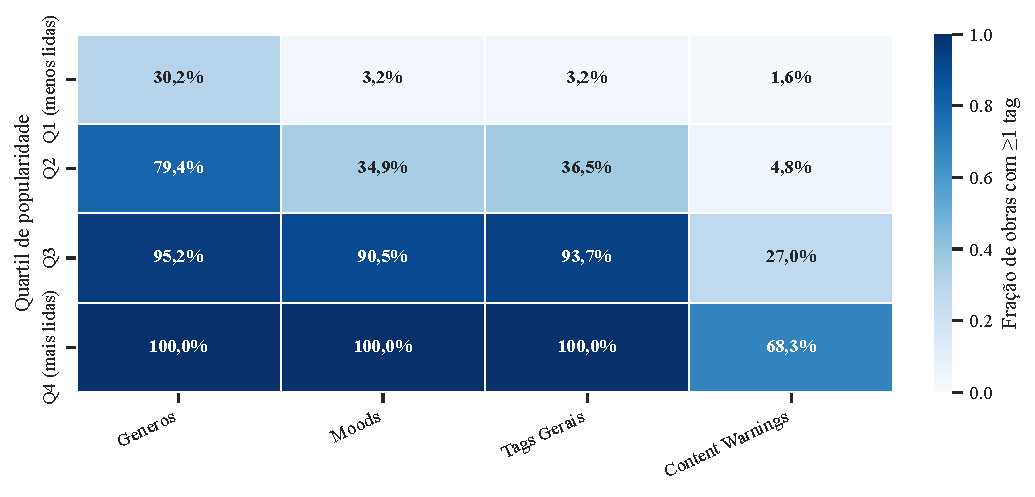
\includegraphics[width=0.8\textwidth]{fig_11_cobertura_popularidade.pdf}
\caption{Fração de obras que têm ao menos uma etiqueta de cada tipo, por grupo de popularidade. Quanto menos lido o livro, menos sabemos sobre ele.}
\label{fig:cobertura}
\end{figure}

\subsection{O que o rótulo diz sobre as 252 obras}
\label{sec:res-rotulo}
Pouco mais de quatro em cada dez obras (107, ou 42\%) receberam o rótulo \emph{alto} --- 66 com evidência forte e 41 com evidência fraca. Dezessete (7\%) foram classificadas como \emph{provavelmente baixo}. E metade (128, ou 51\%) ficou \emph{indeterminada} (Figura~\ref{fig:label}). Esse último número não é uma falha do método; é o método funcionando. Os indeterminados concentram-se nos grupos menos lidos (104 dos 128 estão na metade menos popular), exatamente onde faltam etiquetas.

Um dado chama a atenção: \textbf{nenhuma obra recebeu o rótulo ``baixo''}. Etiquetas que indicariam explicitamente um livro leve (\emph{closed door}, \emph{clean romance}) simplesmente não ocorrem na amostra. Isso revela algo sobre a cultura das plataformas --- leitores avisam sobre o que há, não sobre o que não há --- e tem uma implicação metodológica que discutimos na Seção~\ref{sec:discussao}: nosso rótulo detecta presença de sinal, nunca ausência de conteúdo.

\begin{figure}[H]
\centering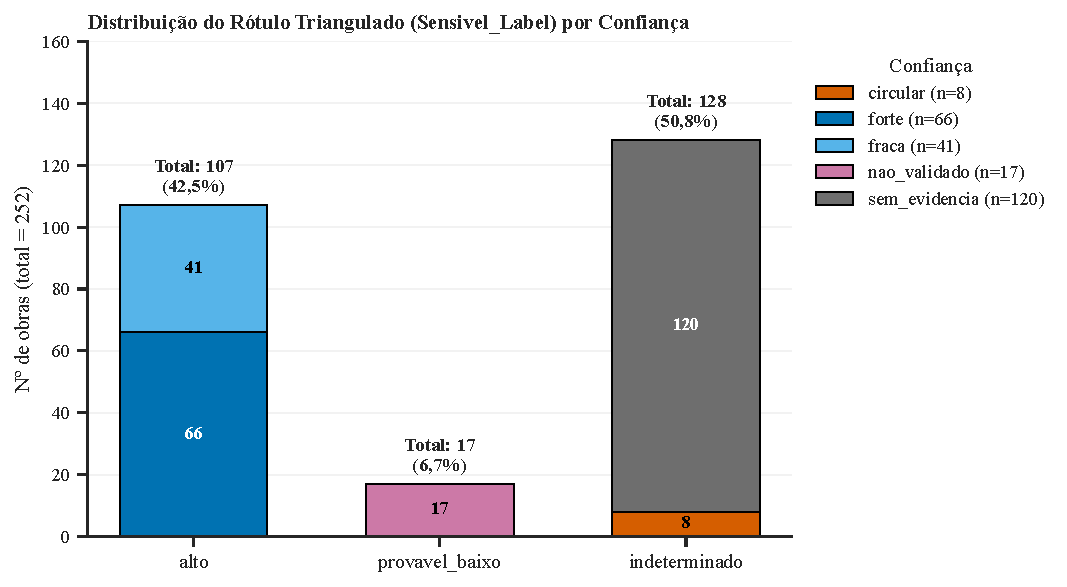
\includegraphics[width=0.85\textwidth]{fig_14_spice_label.pdf}
\caption{Distribuição do rótulo nas 252 obras, por grau de confiança.}
\label{fig:label}
\end{figure}

A proporção de obras \emph{alto} sobe de 11\% no grupo menos lido para 81\% no mais lido (Figura~\ref{fig:pop}). Seria tentador concluir que livros populares são mais explícitos. Parte disso pode ser verdade, mas parte é apenas o efeito da Seção~\ref{sec:res-mnar}: nos livros populares, o conteúdo sensível é \emph{visível}; nos demais, pode existir sem ser registrado. Separar os dois efeitos exigirá a validação humana.

\begin{figure}[H]
\centering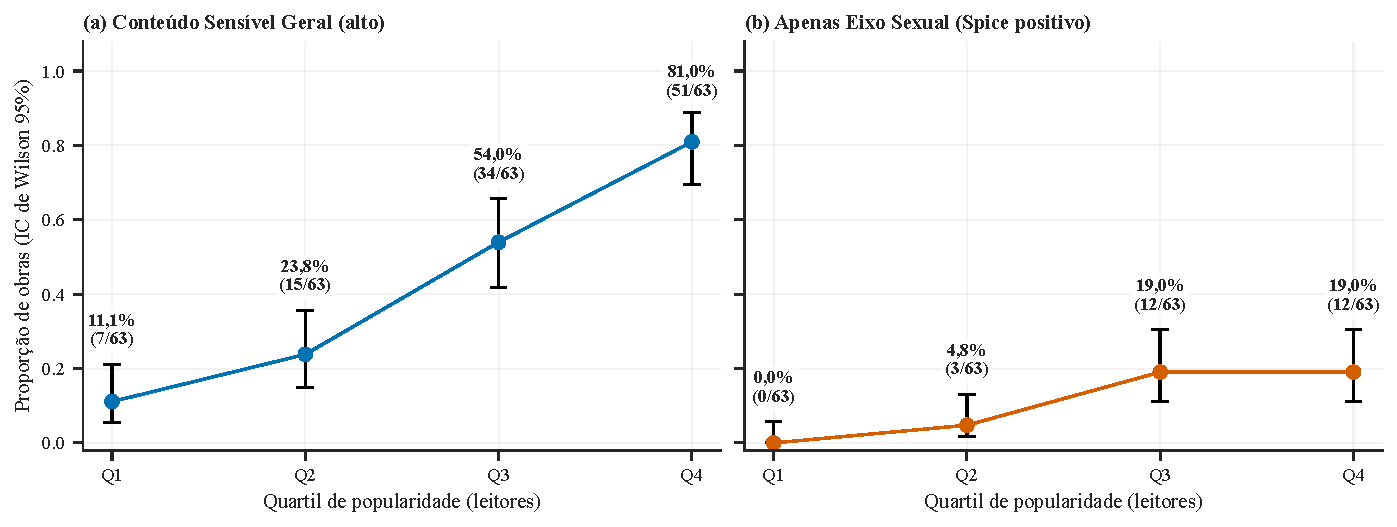
\includegraphics[width=0.95\textwidth]{fig_12_spice_vs_popularidade.pdf}
\caption{Proporção de obras com rótulo \emph{alto} (a) e com sinal erótico explícito (b), por grupo de popularidade. As barras verticais indicam a incerteza estatística.}
\label{fig:pop}
\end{figure}

\subsection{Quais eixos aparecem, e como se combinam}
Olhando eixo a eixo (Figura~\ref{fig:eixos}), cerca de quatro em cada dez obras (98, ou 39\%) apresentam algum sinal sensível. O eixo mais frequente é, como esperado para romances, o sexual (um terço das obras). Mas violência e abuso aparecem cada um em cerca de 15\% das obras, e drogas e álcool em 7\% --- frequências nada desprezíveis para livros vendidos com capas juvenis. E os eixos raramente vêm sozinhos: metade das obras sensíveis acumula dois ou mais, com a combinação ``sexo + violência + abuso'' sendo a segunda mais comum (Figura~\ref{fig:cooc}). ``Conteúdo sensível'', portanto, não é uma coisa só, e um estudo que olhasse apenas para o erotismo perderia boa parte do quadro.

\begin{figure}[H]
\centering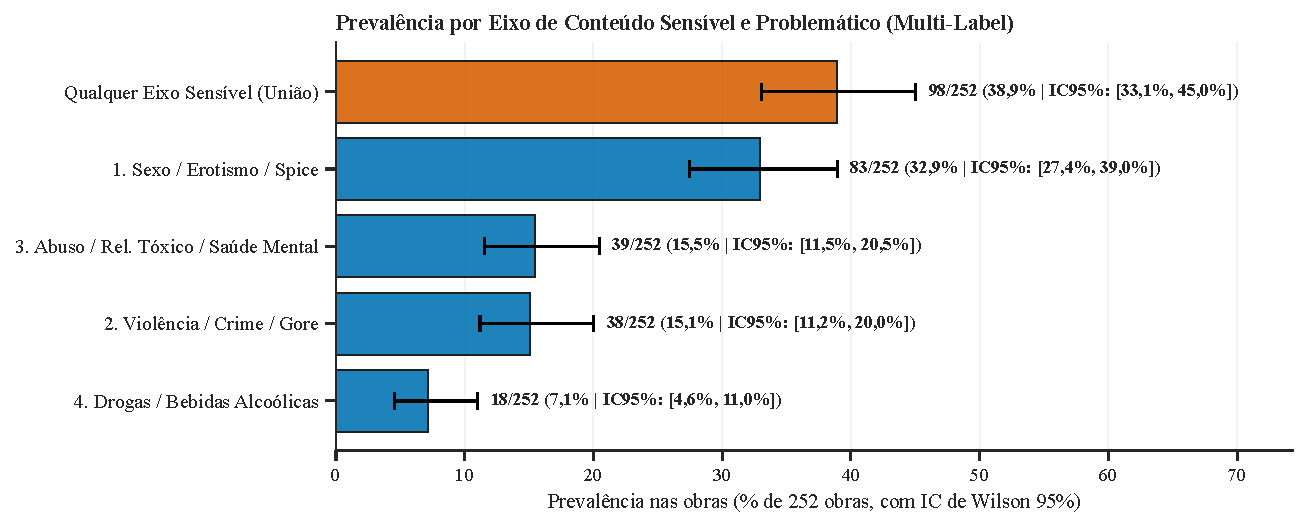
\includegraphics[width=0.95\textwidth]{fig_15_eixos_sensiveis.pdf}
\caption{Quantas obras apresentam cada eixo de conteúdo sensível. Uma obra pode contar em mais de um eixo.}
\label{fig:eixos}
\end{figure}

\begin{figure}[H]
\centering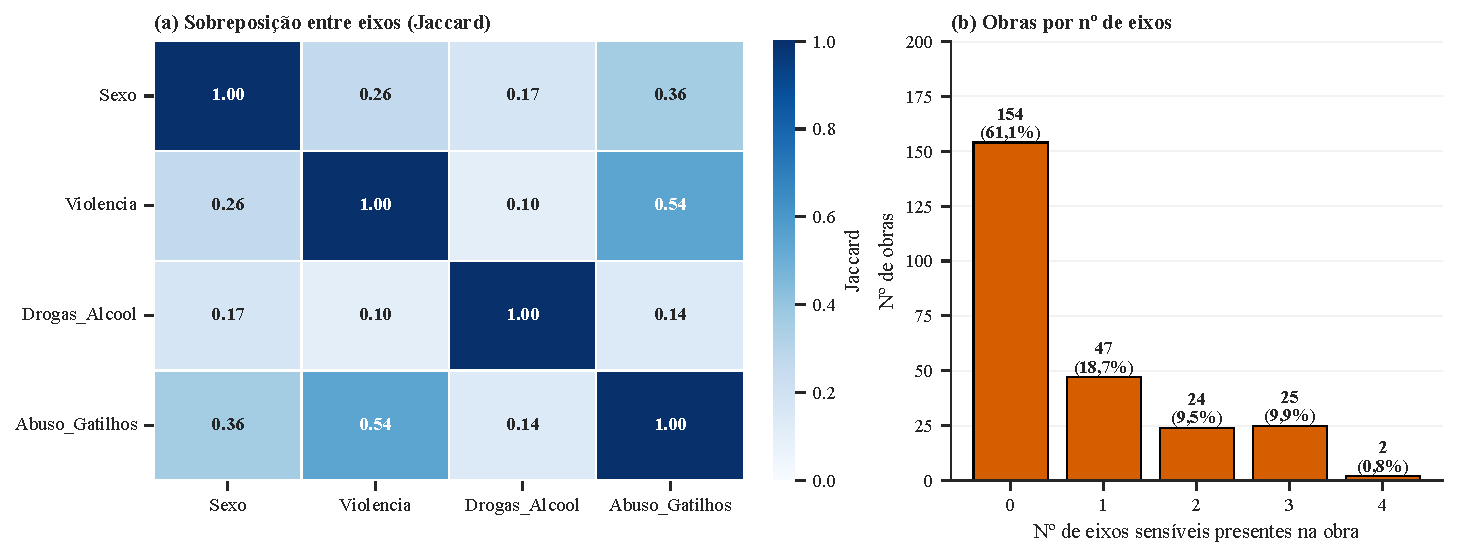
\includegraphics[width=0.95\textwidth]{fig_18_coocorrencia.pdf}
\caption{(a) Quanto os eixos se sobrepõem; (b) quantas obras têm um, dois, três ou quatro eixos ao mesmo tempo.}
\label{fig:cooc}
\end{figure}

\subsection{A sinopse não avisa}
\label{sec:res-omissao}
Este é o resultado mais diretamente ligado à motivação do trabalho. Tomamos as 61 obras em que os leitores registraram algum alerta de conteúdo e perguntamos: a sinopse brasileira menciona esse tema? Em 42 delas (69\%), não --- nenhuma palavra do vocabulário correspondente aparece. Por eixo, o silêncio é ainda mais eloquente (Figura~\ref{fig:omissao}): a sinopse omite o tema em três de cada quatro livros com alerta sexual, em mais de nove em cada dez com alerta de violência ou de abuso, e em \emph{todos} os dezoito livros com alerta de drogas ou álcool.

É preciso cautela na interpretação: nosso vocabulário em português pode não capturar todas as formas de mencionar um tema, e a sinopse não tem a obrigação de ser um aviso de conteúdo. Ainda assim, o padrão é consistente e forte. Ele confirma, com números, a premissa de que o leitor que decide pela capa e pela sinopse decide com informação incompleta --- e sugere que a omissão é maior justamente nos temas menos ``vendáveis''.

\begin{figure}[H]
\centering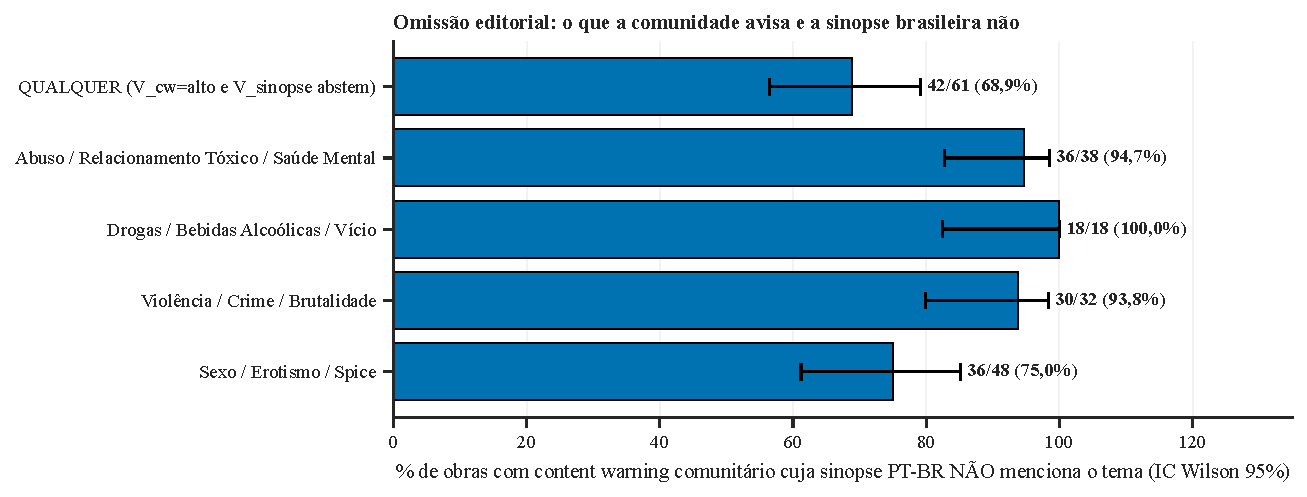
\includegraphics[width=0.95\textwidth]{fig_19_omissao_editorial.pdf}
\caption{Entre as obras que os leitores marcaram com alerta de cada tipo, a fração cuja sinopse brasileira não menciona o tema.}
\label{fig:omissao}
\end{figure}

\subsection{O rótulo é robusto?}
\label{sec:res-robustez}
Removendo uma fonte de evidência por vez, descobrimos quem sustenta o rótulo (Figura~\ref{fig:ablacao}). As etiquetas de gênero e vocabulário quase não fazem diferença. A sinopse muda o rótulo de 9 obras; a classificação etária, de 22. Os alertas de conteúdo dos leitores são de longe a fonte mais importante: sem eles, as decisões ``fortes'' caem de 66 para 15. Por outro lado, nenhuma fonte isolada reproduz o resultado completo --- a melhor delas, sozinha, erra em 46 obras. É o argumento empírico para combinar fontes em vez de escolher uma.

Variando os parâmetros de decisão, o número de obras \emph{alto} não se altera, como esperado; apenas o rótulo \emph{provavelmente baixo}, por ser uma inferência, oscila entre 8 e 19 obras conforme o limiar de popularidade. Reportamos essa variação para que o leitor saiba que ela existe.

Por fim, nas 48 obras em que duas ou mais fontes se manifestaram, \emph{todas} concordaram. Isso parece ótimo, mas é enganoso: concordaram porque todas disseram ``alto''. Nunca houve uma fonte dizendo ``baixo'' para outra discordar. É mais uma face do mesmo fato --- o sistema não tem um polo negativo mensurável.

\begin{figure}[H]
\centering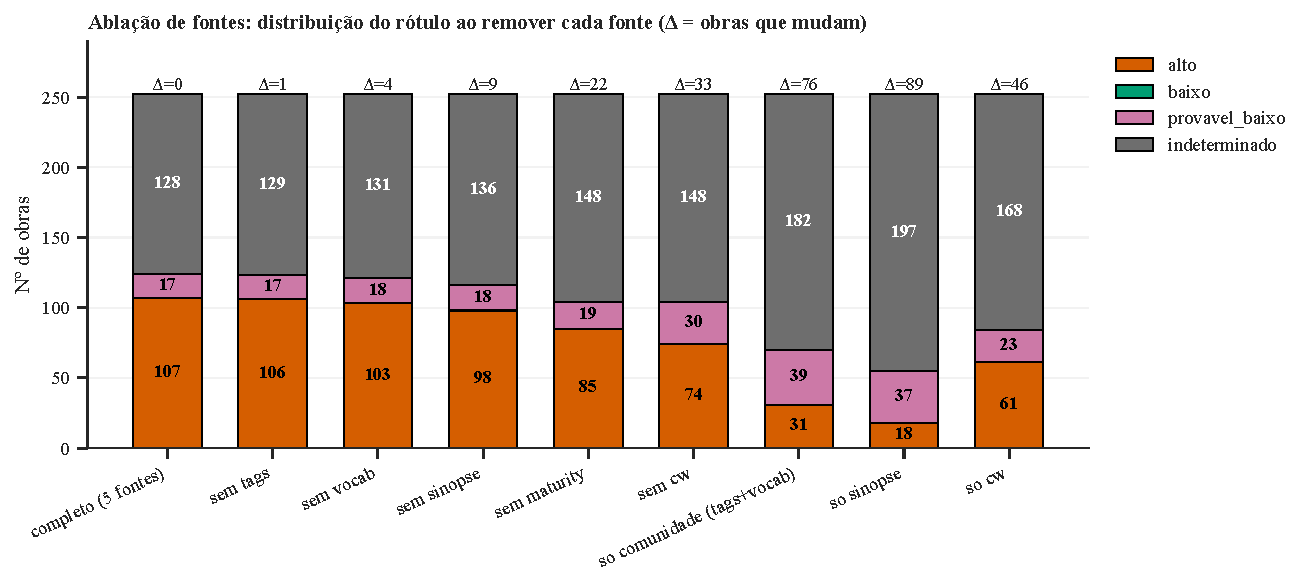
\includegraphics[width=0.95\textwidth]{fig_17_ablacao.pdf}
\caption{O que acontece com o rótulo quando removemos cada fonte de evidência. $\Delta$ indica quantas obras mudam de rótulo.}
\label{fig:ablacao}
\end{figure}

\subsection{Validação humana}
\label{sec:res-gold}
\emph{(Em andamento. Esta seção reportará quanto os dois anotadores concordaram entre si, com que frequência o rótulo automático coincidiu com o julgamento humano, eixo por eixo, e qual a precisão da ligação edição--obra conferida manualmente.)}

% =========================================================================
\section{Discussão: o que esta base pode e não pode dizer}
\label{sec:discussao}

\subsection{Como ler o rótulo}
O rótulo \emph{alto} significa ``há evidência convergente de conteúdo sensível''. O rótulo \emph{indeterminado} significa ``não há evidência'' --- e isso inclui tanto livros realmente leves quanto livros sensíveis que ninguém marcou. O rótulo \emph{provavelmente baixo} é uma aposta informada, não uma constatação, e usá-lo como se fosse um ``negativo confirmado'' em um estudo de capas seria raciocinar em círculo: estaríamos assumindo que capa juvenil implica conteúdo leve, que é precisamente a hipótese que queremos testar. Em termos técnicos, a base é \emph{positive-unlabelled}: serve para estudar o que tem sinal, não para afirmar o que não tem.

\subsection{Limites}
\textbf{Popularidade confunde.} Como vimos, livros populares têm mais etiquetas e, por isso, mais rótulos \emph{alto}. Qualquer análise futura que relacione capa e conteúdo precisa controlar a popularidade, sob pena de ``descobrir'' que capas de livros famosos são mais discrepantes apenas porque sabemos mais sobre livros famosos.

\textbf{A amostra não é o mercado.} Perdemos mais da metade das edições na ligação com o Hardcover, e perdemos de forma desigual: autoras nacionais, autopublicação e livros de nicho estão sub-representados. Os números aqui descrevem a base construída, não o mercado editorial brasileiro.

\textbf{O vocabulário é uma escolha.} Os quatro eixos e seus termos foram definidos por nós. É possível que o eixo de drogas e álcool, o menos frequente e o mais omitido pela sinopse, seja também o mais mal coberto pelo nosso vocabulário em português. A validação humana ajudará a estimar isso.

\textbf{Buscamos o que queríamos achar.} Um dos caminhos de coleta usou termos de conteúdo adulto. Neutralizamos o efeito disso na sinopse, mas essas obras continuam na base. Sem elas, o rótulo \emph{alto} cai de 107 para 79 obras --- a direção dos resultados não muda, mas a magnitude depende da amostra.

\subsection{Implicações para a próxima etapa}
A base oferece, para cada edição, capa validada, sinopse, rótulo em quatro eixos e dois alvos (com e sem sinopse). A próxima etapa --- comparar a estética da capa com o conteúdo --- deve comparar livros com rótulo \emph{alto} contra livros confirmados como leves por pessoas, nunca contra os indeterminados; deve tratar a popularidade como variável de controle; e deve considerar métodos adequados a dados em que só o lado positivo é observado.

% =========================================================================
\section{Conclusão}
\label{sec:conclusao}
Partimos de uma pergunta simples --- capas juvenis estão sendo usadas para vender conteúdo adulto? --- e descobrimos que, antes de respondê-la, era preciso resolver um problema anterior: não existia uma forma confiável e independente da editora de saber o que um livro brasileiro contém. Construímos essa forma. O processo liga edições brasileiras às obras originais, lê o que milhares de leitores registraram sobre elas e combina essa informação com cautela, admitindo não saber quando não sabe.

No caminho, dois achados se impõem. O primeiro é que a sinopse brasileira silencia sobre a maior parte do que os leitores consideram digno de alerta --- em alguns temas, sobre tudo. Isso dá substância à preocupação que motivou o trabalho. O segundo é que a informação disponível sobre um livro é proporcional à sua fama, o que obriga qualquer estudo nessa área a distinguir ``não tem'' de ``não sabemos''. Com a base construída e suas limitações mapeadas, a próxima etapa --- olhar para as capas --- pode começar em terreno firme.

% -------------------------------------------------------------------------
\section*{Disponibilidade}
Código, vocabulário, tabelas e figuras estão em \url{https://github.com/hellolima/mismatch-analysis}.

% -------------------------------------------------------------------------
\appendix
\section{Detalhes técnicos e dicionário de dados}
Os limiares da ligação edição--obra, as oito regras de decisão do rótulo e a descrição de cada coluna da base estão no documento \texttt{ARQUITETURA\_E\_PIPELINE.md} do repositório e nas tabelas \texttt{regras\_decisao.csv} e \texttt{aval\_*.csv}. \emph{(Reproduzir aqui a tabela de regras e as tabelas numéricas de ablação e sensibilidade.)}

\section{Vocabulário completo dos quatro eixos}
Gerado automaticamente em \texttt{outputs/tables/lexico\_eixos.csv} (130 termos). \emph{(Importar como tabela.)}

\section{Protocolo de anotação humana}
Ver \texttt{data/gold\_standard/PROTOCOLO\_ANOTACAO.md}. \emph{(Reproduzir.)}

% -------------------------------------------------------------------------
\begin{thebibliography}{99}
\bibitem{TODO-design-capas} \textsc{[A completar]} Design de capas como sinal de gênero e público.
\bibitem{TODO-clickbait} \textsc{[A completar]} \emph{Clickbait} e \emph{thumbnails} enganosas.
\bibitem{TODO-exposicao-conteudo} \textsc{[A completar]} Exposição de menores a conteúdo inadequado.
\bibitem{TODO-lei15211} Brasil. Lei nº 15.211, de 2025. Estatuto Digital da Criança e do Adolescente.
\bibitem{TODO-social-media-livros} \textsc{[A completar]} BookTok e o mercado editorial.
\bibitem{TODO-frbr} IFLA. \emph{Functional Requirements for Bibliographic Records}; IFLA Library Reference Model.
\bibitem{TODO-record-linkage} Christen, P. \emph{Data Matching}. Springer, 2012.
\bibitem{TODO-folksonomia} \textsc{[A completar]} Folksonomia e catalogação social.
\bibitem{TODO-weak-supervision} Ratner, A. et al. Snorkel: rapid training data creation with weak supervision. \emph{VLDB}, 2017.
\bibitem{TODO-pu-learning} Bekker, J.; Davis, J. Learning from positive and unlabeled data: a survey. \emph{Machine Learning}, 2020.
\bibitem{TODO-mnar} Little, R.; Rubin, D. \emph{Statistical Analysis with Missing Data}. Wiley, 3.\ ed., 2019.
\bibitem{TODO-cover-genre} \textsc{[A completar]} Classificação de gênero a partir de capas de livros.
\bibitem{TODO-age-text} \textsc{[A completar]} Predição de faixa etária a partir de texto.
\bibitem{TODO-goodreads-api} \textsc{[A completar]} Descontinuação da API do Goodreads (2020).
\end{thebibliography}

\end{document}